Le graphe cellule $G_{k,k'}$ ne contient aucune clique. 
Nous appliquons l'algorithme de correction pour cr\'eer des cliques qui couvrent les sommets de ${\cal C}$ et dont le line-graphe propos\'e est de distance minimale.
Pour effectuer la correction, nous pouvons soit ajouter ou soit supprimer des ar\^etes uniquement.
Soient la fonction de co\^ut {\em ajout} qui ajoute uniquement des ar\^etes et la fonction de co\^ut {\em suppression} qui supprime uniquement des ar\^etes. 
Nous allons d\'etailler les op\'erations d'ajout et de suppression d'ar\^etes pendant l'algorithme de correction. 

\subsubsection{Correction avec la fonction {\em ajout}}
Soit le graphe $G_{k,k'}$ contenant $k \times k' + 1$ cellules.
Pour transformer chaque cellule en cliques, nous devons ajouter $2$ ar\^etes.
Nous consid\'erons le sommet $(0,0)$ contenu dans les cellules $G_{0,0}$ et $G_{k,k'}$.
Nous ajoutons $2$ ar\^etes dans $G_{0,0}$ et $G_{k,k'}$. Les cellules deviennent des cliques $K_4$. 
\newline
L'ar\^ete $\{(0,1),(1,1)\}$ appartient aux cellules  $G_{0,0}$ et  $G_{0,1}$. Or cette ar\^ete est d\'ej\`a couverte par une clique $K_4$ de la cellule $G_{0,0}$. Alors nous ne pouvons pas ajouter d'ar\^etes dans la cellule $G_{0,1}$. L'ar\^ete $\{(0,1),(0,2)\}$ forme une clique $K_2$. Le sommet $(0,1)$ est couvert par une clique $K_4$ et une clique $K_2$. 
Le sommet $(1,0)$ est aussi couvert par une clique $K_4$ et une clique $K_2$ parce que les cellules $G_{0,0}$ et  $G_{1,0}$ partagent l'ar\^ete $\{(1,0),(1,1)\}$  et cette ar\^ete forme une clique $K_4$ avec la cellule $G_{0,0}$.
Les $G_{0,0}$ et  $G_{1,1}$ ne partagent que le sommet  $(1,1)$. En plus les ar\^etes  $\{(1,1),(2,1)\}$ de  $G_{1,0}$ et  $\{(1,1),(1,2)\}$ de $G_{0,1}$ ne sont pas couverts par une clique $K_4$. Nous pouvons alors transformer $G_{1,1}$ en une clique $K_4$  en ajoutant $2$ ar\^etes .
\newline
Ainsi, dans les cellules cons\'ecutives quelle que soit la ligne (avec $k$) et la colonne (avec $k'$), nous ajoutons des ar\^etes dans une cellule sur deux. 
%Une ar\^ete d'une cellule dans laquelle nous n'avons pas ajout\'e d'aretes devient une clique $K_2$. 
L'ar\^ete  d'une cellule qui n'est pas contenue par une clique $K_4$ forme une clique $K_2$.
Les cellules ayant un seul sommet en commun sont transform\'ees en des cliques $K_4$. 
\newline
\`A la fin  de la correction, le graphe cellule $G_{k,k'}$ est partitionn\'e par des cliques $K_4$ et $K_2$.
La distance de Hamming entre $G_{k,k'}$ et $L(G_{k,k'})$ est de $DH_{k,k'} = 2 \times (\lceil \frac{k \times k'}{2} \rceil  + 1)$ et cette distance est minimale.
\begin{theorem}
La distance line d'un graphe cellule $G_{k,k'}$ avec la fonction {\em ajout} est 
\begin{equation}
DL_{ajout}(G_{k,k'}) = 2 \times (\lceil \frac{k \times k'}{2} \rceil  + 1)
\end{equation}
\end{theorem}

% ---- figure exemple correction graphe cellule G_{3,3}
\begin{figure}[htb!] 
\centering
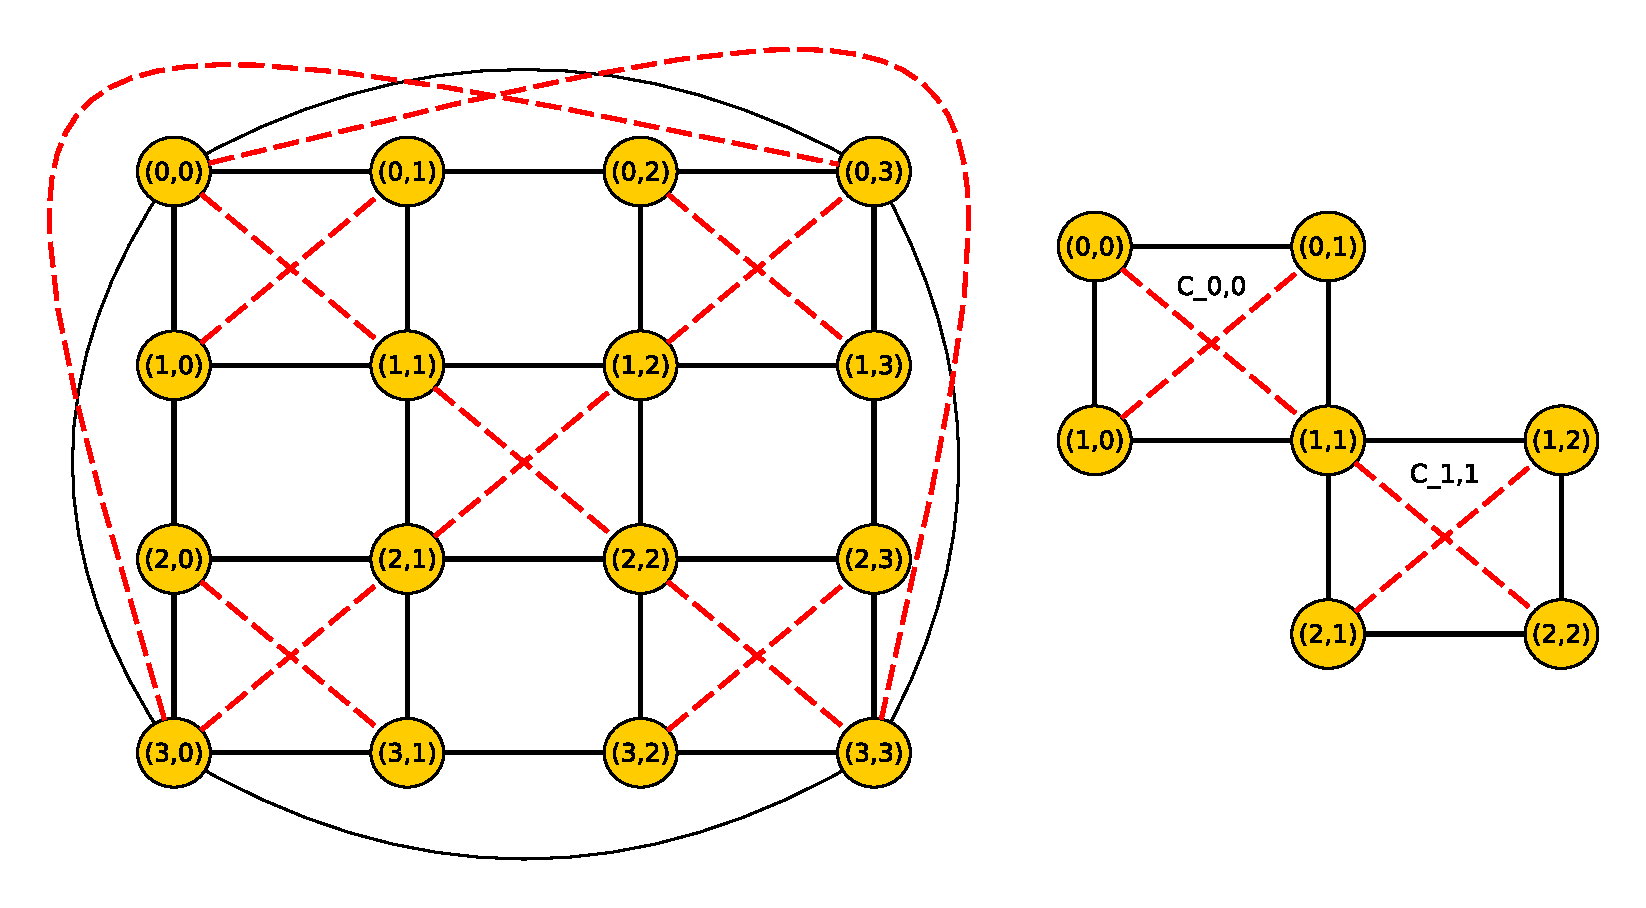
\includegraphics[scale= 0.7]{exempleGrapheCelluleAjoutG33.eps}
\caption{ Le graphe cellule $G_{3,3}$ : il est compos\'e de $16$ sommets, $33$ ar\^etes. Il contient $4$ cliques $K_{2}$ et $6$ cliques $K_4$. Les ar\^etes ajout\'ees sont les traits de couleur rouge.}
\label{exempleCorrectionGrapheCelluleAvecAjout}
\end{figure}
% ---- figure exemple correction graphe cellule G_{3,3}
Dans la figure \ref{exempleCorrectionGrapheCelluleAvecAjout}, nous r\'ealisons la correction de distance line minimale en transformant les cellules partageant un sommet en cliques $K_4$. C'est le cas des cellules $G_{1,2}$ et  $G_{0,2}$ qui ont le sommet $(1,2)$ en commun. 
Les ar\^etes partag\'ees entre deux cellules ont un des sommets couvert par une clique $K_2$ et l'autre sommet couvert par une clique $K_4$. Tel est le cas avec le sommet $(3,2)$ qui forme l'ar\^ete $\{(2,2),(3,2)\}$ et cette ar\^ete est contenue par une clique $K_4$.

\subsubsection{Correction avec la fonction {\em suppression}}
Soit le graphe $G_{k,k'}$ contenant $k \times k' + 1$ cellules.
Pour transformer chaque cellule en cliques, nous devons supprimer $3$ ar\^etes dans la cellule $G_{k,k'}$ et $1$ ar\^ete dans les autres cellules.
Nous consid\'erons un sommet  de degr\'e minimun par exemple$(0,1)$. Ce sommet appartient \`a $2$ cellules  $G_{0,0}$ et $G_{0,1}$. Pour que le sommet $(0,1)$ soit couvert par $2$ cliques de cellules diff\'erentes, nous supprimons l'ar\^ete $\{(0,1),(1,1)\}$ et nous formons ainsi $2$ cliques $K_2$ dans chacune des cellules. 
\newline
Ensuite, en consid\'erant les sommets de degr\'e minimum \`a chaque correction de sommet, nous supprimons les ar\^etes verticales dans chaque ligne. 
Par exemple, les ar\^etes $\{(0,3),(1,3)\}$ et $\{(0,4),(1,4)\}$ entre respectivement les cellules $G_{0,2}$ et  $G_{0,3}$ et  les cellules $G_{0,3}$ et  $G_{0,4}$ sont supprim\'ees. Ainsi les cellules de chaque ligne ne partagent aucune ar\^ete entre elles et chaque cellule ne contient que $2$ ar\^etes verticales. Ces $2$ ar\^etes forment $2$ cliques $K_2$.
\newline
Il nous reste que les sommets de degr\'e $4$. Les ar\^etes formant des cliques $K_2$  et incidentes \`a un tel sommet sont conserv\'ees et les autres ar\^etes sont supprim\'ees.  Par exemple, prenons le sommet $(0,0)$ qui est couvert par $2$ cliques $K_2$ ($\{(0,0),(1,0)\}$ et $\{(0,0),(0,1)\}$). Nous supprimons les ar\^etes  $\{(0,0),(0,k'+1)\}$ et $\{(0,0),(k+1,0)\}$).
\newline
Pour les sommets \'etant couverts par une clique $K_2$, nous supprimons les ar\^etes verticales des cellules dont ils appartiennent. Par exemple, en s\'electionnant le sommet $(0,k'+1)$, il est d\'ej\`a couvert par la clique $K_2 = \{(0,k'),(0,k'+1)\}$ et l'ar\^ete $\{(0,0),(0,k'+1)\}$ a d\'ej\`a \'et\'e supprim\'ee. Nous supprimons l'ar\^ete  $\{(0,k'+1), (1, k'+1)\}$ et le sommet  $(0,k'+1)$ est alors couvert par $2$ cliques $K_2$ ($\{(0,k'),(0,k'+1)\}$ et $(0,k'+1),(k+1,k'+1)$).
\newline
Cette op\'eration de correction est aussi correcte si nous supprimons les ar\^etes horizontales dans chaque colonne. 
\newline
\`A la fin de l'algorithme de correction, le graphe $G_{k,k'}$ est partitionn\'e avec des cliques $K_2$ et ce graphe est un cycle de taille $(k \times k'+1) + k' + 1$.
La distance de Hamming   entre $G_{k,k'}$ et $L(G_{k,k'})$ est $DH_{k,k'} = k \times k' +3 $ et cette distance est minimale.

\begin{theorem}
La distance line  d'un graphe cellule $G_{k,k'}$ avec la fonction {\em suppression} est 
\begin{equation}
DL_{supp}(G_{k,k'}) = k \times k' +3 
%DL_{supp}(G_{k,k'}) = k \times (k' +1) ===> cela correspond a quoi?
\end{equation}
\end{theorem}

% ---- figure exemple correction graphe cellule G_{3,3}
\begin{figure}[htb!] 
\centering
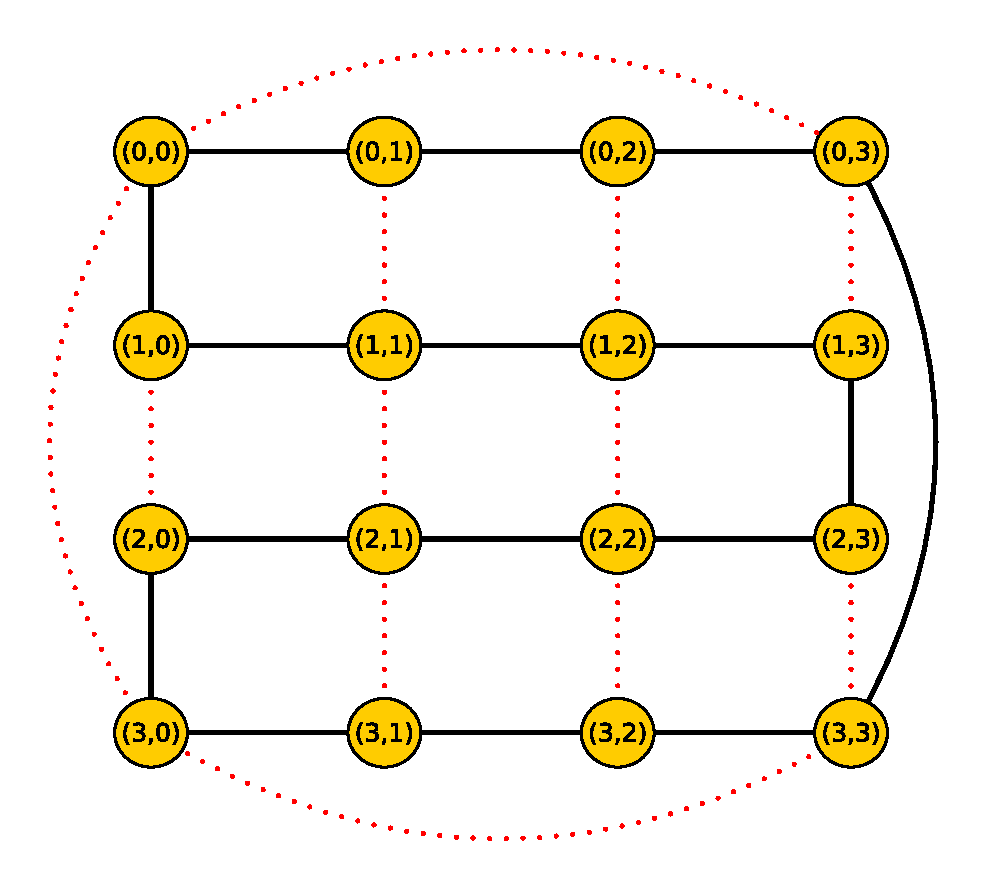
\includegraphics[scale = 0.7]{exempleGrapheCellulesSuppressionG33.eps}
\caption{ Le graphe cellule $G_{3,3}$ : il est compos\'e de $16$ sommets, $16$ ar\^etes et $16$ cliques $K_2$. Les ar\^etes supprim\'ees sont les traits en pointill\'ees rouges }
\label{exempleCorrectionGrapheCelluleAvecSuppression}
\end{figure}
% ---- figure exemple correction graphe cellule G_{3,3}
Une illustration de la correction avec la fonction suppression est faite avec le graphe $G_{3,3}$ dans la figure \ref{exempleCorrectionGrapheCelluleAvecSuppression}.
Le graphe $G_{3,3}$ poss\`ede $(k+1)\times (k'+1) = 16$ cliques $K_2$ et $12$ ar\^etes sont supprim\'ees.
\newline

% conclusion
Nous avons d\'etermin\'e les distances line th\'eoriques selon les fonctions de co\^ut lors de la correction de sommets de graphes cellules. Nous allons v\'erifier si les distances line obtenues exp\'erimentalement convergent vers les distances line th\'eoriques.





